\documentclass{article}
\usepackage[utf8]{inputenc}
\usepackage{amssymb}
\usepackage{amsthm}
\usepackage{amsmath}
\usepackage{epic}
\usepackage{eepic}
\usepackage{paralist}
\usepackage{listings}
\usepackage{graphicx}
\usepackage{algorithm,algorithmic}
\usepackage{tikz}
\usepackage{xcolor,colortbl}
\usepackage{wrapfig}
\usepackage{xcolor}
\usepackage[margin = 1 in]{geometry}

\usepackage{hyperref}


%New colors defined below
\definecolor{codeblue}{rgb}{0,0.1,0.9}
\definecolor{codegreen}{rgb}{0,0.5,0}
\definecolor{codegray}{rgb}{0.5,0.5,0.5}
\definecolor{codeyellow}{rgb}{0.5,0.5,0}
\definecolor{backcolour}{rgb}{1.0,1.0,1.0}

%Code listing style named "mystyle"
\lstdefinestyle{mystyle}{
backgroundcolor=\color{backcolour},   commentstyle=\color{codeyellow},
keywordstyle=\color{codeblue},
numberstyle=\tiny\color{codegray},
stringstyle=\color{orange},
basicstyle=\ttfamily \normalsize,
breakatwhitespace=false,
breaklines=true,
captionpos=b,
keepspaces=true,
lineskip=0.2em,
numbers=left,
numbersep=5pt,
showspaces=false,
showstringspaces=false,
showtabs=false,
tabsize=2
}

%"mystyle" code listing set
\lstset{style=mystyle}


\title{CS5220: Shallow Water Project}
\author{Junyoung Lim (jl3248), Cheng Perng Phoo(cp598), Robert Stephany (rrs254)}
\date{November 3, 2020}

\begin{document}

\maketitle

\section{Introduction}

In this project, we parallelized a finite volume solver for the shallow water equations on a rectangular grid with periodic boundary conditions.
We also explored ways to optimize and tune the parallel solver.
Our implementation is based on a finite volume solver for 2D hyperbolic PDEs
via a high-resolution finite difference scheme by \href{http://www.cscamm.umd.edu/tadmor/pub/central-schemes/Jiang-Tadmor.SISSC-98.pdf}{Jiang and Tadmor}.
Our approach is built upon two central themes: sub-domain partitioning and parallelization using OpenMP.
Based on the performance analysis, our final approach achieved an almost three-fold speedup over a tuned serial implementation.
In particular, we observed a twofold speedup on two processors (See \ref{sec: strong_scaling}).
Our implementation can be found at: \url{https://github.com/cpphoo/shallow-water}.

\section{Sub-domain Partitioning}
\label{sec:subdomain_partitioning}
In this section, we focus on the high-level implementation logic.
We defer details on OpenMP parallelization to the next section (section \ref{sec: parallelization}).
Throughout this report, we will let $U_G$ denote the global grid of cells upon which we want to simulate the shallow water equations.
$U_G$ is partitioned into $N$ sub-grids $\{U_i\}_{i=1}^N$.
A team of $N$ threads solves the shallow water equations on the subgrids (each thread gets a subgrid).

\subsection{Maintaining Sub-grids Consistency Via a Global Grid $U_G$}

The underlying PDE solver updates the water height and momentum in a cell using the corresponding values in each of the four cells which border it.
This means that, for a thread to update the cells on the border of its subdomain,  it must be able to access must access cells outside of its sub-grid.
Fortunately, however, this also means that each thread only needs access to the cells which are adjacent to the boundary of its sub-grid.
To ensure that each thread has access to the information it needs to update its boundary cells, we pad each $U_i$ with a few layers of ``ghost'' cells.
The ghost cells essentially hold copies of the cells (from other sub-grids) that the thread needs to update its sub-grid.
We periodically update the ghost cells using the global grid $U_g$, which acts as a shared repository through which the threads can communicate.

When the threads update their ``ghost'' cells, they first push the first and last few rows and columns of their sub-grid to their corresponding locations in the global grid
(we do this because the other threads will need access to these cells when updating their ghost cells).
Once this finishes, we apply periodic boundary conditions to $U_G$.
After that, each thread updates the momentum and water height in its ``ghost'' cells the values in the corresponding cells in the global grid (which, at this point, have been updated by the other threads).
This order of operation ensures that the periodic BCs are applied and that each thread's ``ghost'' cells are consistent enough with the cells (in other sub-grids) that they correspond to for the thread to correctly update its sub-grid.

\subsection{Determining $dt$ for Finite Difference}
Once we have applied the boundary conditions are applied and each thread has updated its ``ghost cells'',
we compute $dt$.
Determining $dt$ in our parallel implementation is trickier than in the serial one.
The serial implementation calculates $dt$ by finding the maximum wave speed across $U_G$.
In our parallel implementation, however, $U_G$ is not updated after each time step.
Thus, in our parallel implementation, each thread finds the maximum wave velocity in its sub-grid $U_i$.
It then uses this maximum to determine $dt_i$, which would be the value of $dt$ necessary to ensure stability on $U_i$.
Once each thread has determined its $dt_i$, we compute $dt$ to be $\min\{dt_i\}_{i=1}^N$ using a shared buffer.
We do this to ensure that each thread uses the same time step and that this time step will give stability on each subgrid.
This approach is equivalent to if a single thread computed the global maximum wave velocity, used that maximum to compute $dt$, and then broadcast $dt$ to the other threads.
Therefore, the value of $dt$ that our approach calculates is the same $dt$ that the serial code would have calculated.
% The rest of the main loop logic were the same as the original work.
% we need to compute the maximum $x$ and $y$ velocities from each local grid and determine $dt_i$ for each $U_i$.
% Once all the computations are done, we determine $dt$ to be $\min\{dt_i\}_{i=1}^N$.
% The rest of the main loop logic were the same as the original work
% , except that we need to make sure that copy the boundary of each local grid to the corresponding
% location in the global grid. Then proceed to the next iteration of the loop only after all the boundaries are copied over.

% This order of operation ensured that the ghost cells of $U_G$ can be easily pulled into those of each $U_i$ Then we can safely apply boundary conditions to each $U_i$ by copying over the relevant cells from $U_G$ into the ghost cells of $U_i$. ghost cells from $U_G$ to $U_i$.


% The


% These ghost cells are periodically updated to ensure that each thread can accurately update its local grid.
% % As in Dr. Bindel's original code, the global grid is also padded with a few layers of ghost cells, but those are used to implement periodic boundary conditions.

% In our implementation, the global grid $U_G$ is used for two purposes: to implement boundary conditions, and to


% Thus, in our approach, the global grid exists, but only a tiny fraction of it is updated at each time step.
%  We decided to keep the global grid for this purpose, and because it allows us to easily write the state of the system at the end of each time frame for visualization purposes.
%  This isn't the most memory-efficient approach, but it doesn't require much communication between the processors and was straight forward to implement in a shared memory environment.


\subsection{Partitioning the Domain}
We set the number of partitions $N$ to be the number of threads running $p$. For simplicity, we decided to split
the grid data row-wise. This allows us to exploit the fact that the grid data (or matrices) follows row-major ordering, thereby improving cache usage when the threads read from and write to $U_G$

% In this section, we explained how the grid were partitioned and provided a few code snippets beneficial for understanding the implementation details discussed in this subsection.
% Interested readers were encouraged to check out our Github repository (\url{https://github.com/cpphoo/shallow-water}) for the full implementation
% which included myriad comments for clear exposition. To start, we set the number of sub-grids $N$ as the number of threads


% we needed to determine the number of subgrids we we would like to create
% In order to apply sub-domain partitioning, we need to determine $N$, the number of partitions to create.
% To generalize our logic, we dynamically determine the number of partitions at runtime by detecting $p$, the number of threads running, and let $N = p$.


% \begin{lstlisting}[language=C]
% // ldriver_parallel.c
% // First get the number of threads from the environment
% // If the number of threads is null, then set the number of threads to 1
% char* s = getenv("OMP_NUM_THREADS");

% int num_threads = 0;
% if (s != NULL) {
%     num_threads = atoi(s);
% }

% if (num_threads == 0) {
%     num_threads = 1;
% }

% printf("Number of threads: %d\n", num_threads);
% const int n_rows = num_threads;
% const int n_cols = 1;
% \end{lstlisting}

% \texttt{n\_row} and \texttt{n\_col}, are used to calculate two variables, \texttt{xlow\_local} and \texttt{ylow\_local}.
% \texttt{xlow\_local} specifies which row of $U_G$ the bottom row of $U_i$ corresponds to. \texttt{ylow\_local} specifies which column of $U_G$ the left column of $U_i$ corresponds to.
% These variables are used to compute the location (\texttt{nx\_local} and \texttt{ny\_local}) in $U_G$ that corresponds to each cell of $U_i$.
% Note that $\texttt{n\_row} = N$ and $\texttt{n\_col} = 1$, because we are exploiting the fact that matrices follow row major ordering in our code. This approach will, therefore, improve cache usage when threads read from and write to $U_g$. We initialize each $U_i$ as shown below.

% \begin{lstlisting}[language=C]
% // ldriver_parallel.c
% float* U_local = sim_local->U;
% float* U = sim -> U;
% for(int k = 0; k < 3; ++k) {  // 3 = nfield
%   for(int iy = 0; iy < ny_local; ++iy) {
%     for(int ix = 0; ix < nx_local; ++ix) {
%       U_local[central2d_offset(sim_local, k, ix, iy)]
%         = U[central2offset(sim, k, xlow_local + ix, ylow_local + iy)];
%     }
%   }
% }
% \end{lstlisting}

% \texttt{stepper\_parallel.c} contains the main logic described in the overview. In addition to the provided functions, we introduce three new functions, each with the following functionalities:

% \begin{itemize}
% 	\item \texttt{central2d\_local\_BC} --- Used to fetch $U_i$'s ghost cells from $U_g$.
% 	\item \texttt{central2d\_local\_to\_global} --- Copies the boundary of $U_i$ back to $U_G$.
% 	\item \texttt{central2d\_U\_to\_global\_U} --- Copies the canonical cells of $U_i$ back to corresponding locations in $U_G$.
% \end{itemize}

\section{OpenMP Parallelization}
\label{sec: parallelization}
Sub-domain partitioning involves handling $N$ disjoint partitions that can be simulated in parallel.
To enable parallelism,
we used a shared memory model.
We implemented this model using OpenMP.
In this section, we elaborate a few key implementations that enables parallelization of sub-domain partitioning.
% \texttt{\#pragma omp} directives are used to ensure proper setup of parallel processing of each thread.

\subsection{Initialization of Each Thread}
Once we determine the number of threads $p$, we initialize each $U_i$ by making a deep copy of partition of the original grid data.
After this, we use the original grid data as our global grid $U_G$. Before the simulation starts, it is crucial to ensure that all threads finish up their $U_i$ initialization.
This is implemented using a barrier. See below for a pseudocode of our thread initialization:

\begin{lstlisting}[language=C]
// ldriver_parallel.c
// n_rows = p
// n_cols = 1
#pragma omp parallel num_threads(n_rows*n_cols)
{
    // use omp_get_thread_num() to compute the sub grid location
    // call central2d_init(...)
    // initialize the U_i for each thread

    // wait for all threads to set up their local arrays.
    #pragma omp barrier
    ...
}
\end{lstlisting}

\subsection{Computing $dt$ via a Shared Buffer}
To update each cell, we need to compute $dt$ for the finite difference. To speed up the computation,
we attempted to parallelize computation as described in section \ref{sec:subdomain_partitioning} which requires a shared
memory buffer. As such, we let the first-arriving thread to create the shared buffer with a single directive
and store its local $dt$ in said buffer. For the rest of the threads, they would update the buffer if their local $dt$ is smaller than
the value stored in the buffer.  We establish a critical section when updating the buffer and set a barrier to wait for all threads
to finish updating the buffer before proceeding. See below for a pseudocode of our implementation:

\begin{lstlisting}[language=C]
// inside central2d_xrun(...) of stepper_parallel.c
    ...
    // calculate dt_local using the data on our partition.

    // Initialize the shared buffer, because the buffer may contain 0.
    #pragma omp single
    {
      shared_buffer[0] = dt_local;
    }

    // Now, each thread writes its data to shared_buffer one by one.
    #pragma omp critical
    {
      shared_buffer[0] = fmin(dt_local, shared_buffer[0]);
    }
    #pragma omp barrier
    ...
\end{lstlisting}

\subsection{Respecting the Boundary Conditions}
After each sub-grid are updated, we copy $U_i$ (on each thread) to the global grid $U_G$ so that
we could apply the periodic boundary conditions on the global grid. To make sure that $U_G$ are completely updated, we again establish
a barrier as shown as follows:

\begin{lstlisting}[language=C]
// inside central2d_xrun(...) of stepper_parallel.c
    ...
    // copy boundary of U to corresponding entries of U global using central2d_local_to_global(...)
    #pragma omp barrier
    ...
\end{lstlisting}

\subsection{Checking for Correctness and Generating Visualization}
The solution check and visualization generation are performed on the global grid $U_G$.

% The following is not necessary since it does not concern performance
% The barrier directive is included so that threads do not start a new time step until every thread has written its boundary data to $U_G$.
% Once the main while loop in \texttt{xrun} completes, each thread writes its $U_i$ into $U_G$.
% We included another \texttt{barrier} directive after this step so that \texttt{xrun} does not return until every thread has finished writing to $U_G$.
% This is done so that, at the end of a time frame, $U_G$ stores the global state of the simulation.
% We can then use $U_G$ to run solution checks and print out to the visualizer.
% A consequence of this is that every thread returns from \texttt{xrun} at the same time.
% Therefore, we can use the time measurement from any one of the cells to evaluate the elapsed time.
% The solution check and visualizer steps can be done independently, and are, therefore, included in a sections directive.
% One section checks the correctness of our solution, and the other writes $U_G$ to the visualizer filer.

% \begin{lstlisting}[language=C]
% // ldriver_parallel.c
% #pragma omp parallel num_threads(n_rows*n_cols)
% {
%     ...
%     #pragma omp barrier

%     for (int i = 0; i < frames; ++i) {
%         // measure time elapsed from central2d_run(...)

%         #pragma omp sections {
%             #pragma omp section {
%               // run out diagnostic on U_i by running solution_check(...)
%             }
%             #pragma omp section {
%               //  write a frame of U to memory by running viz_frame(...);
%             }
%         }
%     }
%     ...
% }
% \end{lstlisting}

\section{Performance Analysis}
In this section, we assume $p$ is the number of threads and each thread is uniquely associated to a processor.

\subsection{Strong Scaling}
\label{sec: strong_scaling}
We performed strong scaling on Graphite. In particular, we set the problem size to be $nx = ny = 1000$ and ran our implementation for $p = 1, 2, 3, \ldots, 10$.
We computed the speedup as $T_{serial} / T_{parallel}$ where $T_{serial}$ was benchmarked using the initial code released to us.
We plotted the speedup against the number of threads in figure \ref{fig:strong_scaling}.
Our strong scaling plot demonstrated a close to linear scaling for the number of threads less than or equal to 5 but the speedup tapered off
as we increased the number of threads due to inparallelizable portion of the code.
Our finding aligned with Amdahl’s Law, i.e, there always exists some code that is inherently serial and hard to parallelize and those serial work upper bound the speedup of parallel code.

\begin{figure}[h!]
	\centering
	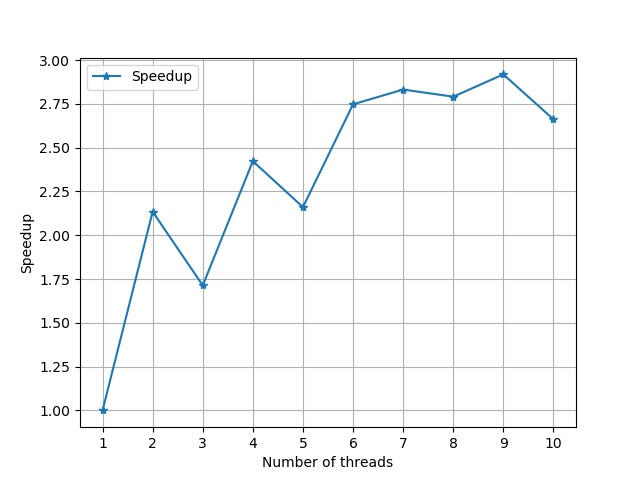
\includegraphics[width=0.8\columnwidth]{../strong_scaling.jpg}
	\caption{Speedup for Strong Scaling Study}
	\label{fig:strong_scaling}
\end{figure}


\subsection{Weak Scaling}
To run weak scaling, we had to scale the problem size with respect to the number of threads such that the amount of work per processor is identical for each thread.
However, this would be be hard to achieve if we wanted to maintain a square grid data.
For instance, suppose we conducted weak scaling on a single thread on a grid of size $h \times h$, then to run weak scaling with 2 threads,
we have to run on a grid of size $2h \times h$ or $h \times 2h$ which was no longer a square grid. As such, we conducted two variants of weak scaling:

\begin{enumerate}
    \item Maintaining the square grid
    \newline
    To make sure that we could conduct weak scaling on a square grid data, we made a compromise by setting the grid’s height and width to be $\lfloor \sqrt{p} \rfloor \times 500$.
    We plot the scaled speedup in figure \ref{fig:weak_scaling}. The scaled speedup hovered around 2 for $p \ge 2$ (the trend line did show that the scaled speedup increased linearly with respect to $p$ but the effect of $p$ is negligible for small $p$).
    Our finding was consistent with Gustafson’s Law, i.e, the scaled speedup is $O(p)$.

    \item Keeping the amount of work per processor identical

    To ensure similar workload for each processor, we conducted weak scaling on grid data of size $500 \times 500p$ (violating the square grid assumption) so that each thread would operate on a grid data of size $500 \times 500$.
    We plotted the scaled speedup in figure \ref{fig:weak_scaling_v2}. Again, we found that the scaled speedup hovered around 2 for $p \ge 2$ with linear dependence with the number of threads.
    Our finding was again consistent with Gustafson’s Law.
\end{enumerate}
\begin{figure}[h!]
	\centering
	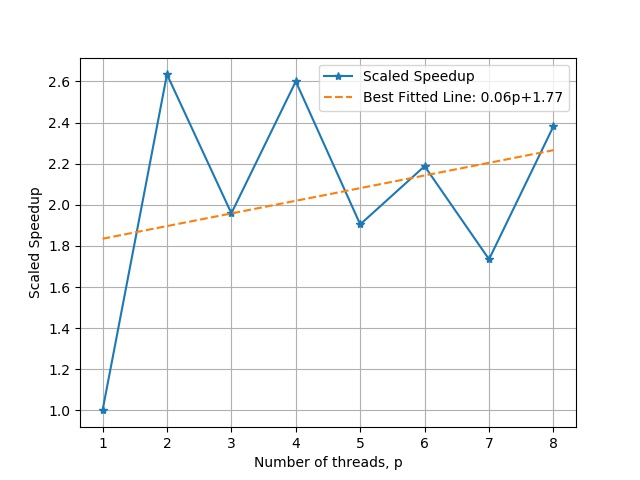
\includegraphics[width=0.8\columnwidth]{../weak_scaling.jpg}
	\caption{Speedup for Weak Scaling (Square Grid)}
	\label{fig:weak_scaling}
\end{figure}

\begin{figure}[h!]
	\centering
	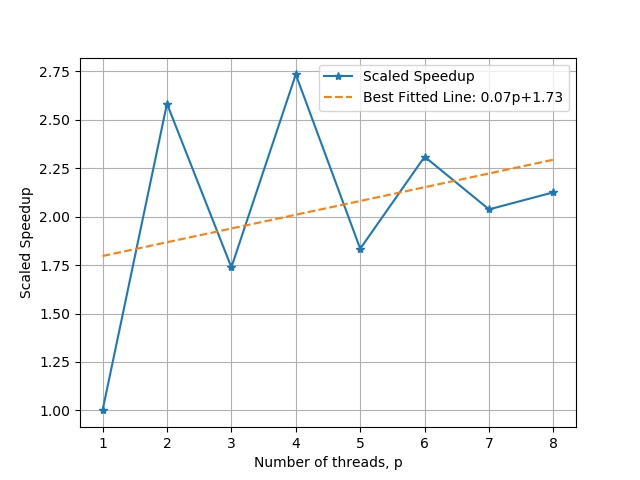
\includegraphics[width=0.8\columnwidth]{../weak_scaling_v2.jpg}
	\caption{Speedup for Weak Scaling (Constant Workload for Processor)}
	\label{fig:weak_scaling_v2}
\end{figure}

\section{Optimization Attempts, Potential Future Improvements}
In this section, we discuss some of the optimizations that we attempted, and discuss changes that we believe could improve our implementation but that we did not have time to implement oursevles.

\subsection{Naively Inserting \text{\#pragma omp parallel}}

We started the project by profiling the serial code provided using gprof (see figure \ref{fig:gprof}) and tried parallelizing a few functions using OpenMP.
In particular, we tried adding \texttt{\#pragma omp parallel for} in three functions: \texttt{central2d\_correct\_sd}, \texttt{shallow\_2dv\_flux} and \texttt{shallow\_2dv\_speed}
but we ended up with an implementation that were significantly slower than the serial code.

\subsection{Parallelizing Periodic BCs}
Our parallel implementation performs most computations in parallel.
However, some steps of our process happen sequentially.
In particular, the Periodic BC's on $U_G$ are applied by a single processor.
We chose this approach initially because it was easy to implement.
In theory, however, this process can happen in parallel.
We tried rewriting \texttt{central2d\_periodic}
with \texttt{parallel for} directives.
This change failed to improve runtime measurably.
We believe that this is because applying the BCs represents a tiny fraction of the overall runtime.
Given these results, we decided to use the serial version of \texttt{central2d\_periodic}.
We chose to do this because we knew that the serial version worked,  would be easier to maintain, and because doing so did not appear to reduce performance.

\subsection{Nested Parallelization}
We also tried adding parallel regions within the predictor/corrector functions of our parallel implementation (these were, therefore, nested parallel regions).
The idea here was that since the code spent most of its runtime in the predictor/corrector methods, and since those methods boil down to big for loops, we might be able to improve performance by having each thread spawn a new team of threads (which we will call `sub-threads') which could run a thread's loops in parallel.
To do this, we tried adding a \texttt{pragma omp parallel for} directive within some of these functions.
This approach failed to improve runtime.
This result makes sense if we consider what's going on.

First, let's consider the case when the number of threads is much less than the number of CPU cores.
In this case, our setup is very similar to the serial case.
As discussed in the previous sub-section, adding parallel for loops to the predictor-corrector methods in the serial implementation failed to improve runtime (probably because the cost of spawning a team of threads outweighed the benefit in parallelization).
Thus, it makes sense that sub-threads in this case also failed to improve runtime.

Now let's consider the case when the number of threads is close to the number of CPU cores.
In this case, there isn't much opportunity for further parallelization.
A thread can spawn a team of sub-threads, but the number of CPU cores stays fixed.
Thus, if there are $N$ cores available, then only $N$ sub-threads can run in parallel.

Given this analysis, it is not surprising that this change failed to improve runtime. After seeing these results, we abandoned this approach and instead focused on trying to use MPI with OpenMP (which is the topic of the next section).

\subsection{Using OpenMP With MPI}
After we got our OpenMP based approach running, we started working on a hybrid OpenMP and MPI strategy.
Via this strategy, we would have used MPI to partition the domain (which in our opinion, is a problem that is better suited for a distributed memory setup)
and OpenMP to further parallelize the computations on each piece of the partition (possibly with a second level of sub-grids).
This approach would allow us to run larger global grids.
One downside to the implementation described above was that it relies on the existence of a global grid that can fit into memory.
If the global grid is too large, it may not be possible to store the entire thing in memory simultaneously.
Our approach with MPI promised to alleviate this bottleneck by eliminating the global grid altogether.

In our MPI based approach, each processor would only hold its local grid.
To make this work, we needed to rewrite our implementation so that it did not rely on a global grid.
As described in previous sections, our implementation used the global grid as a repository through which the threads could communicate, apply global periodic boundary conditions, run the solution check, and simplify the visualizer code.
Switching to MPI, therefore, required us to implement these features without a global grid.

Some of these features were natural to implement in MPI.
For example, to communicate between processors, we could have the processors send their boundary data directly to one another rather than using the global grid as a buffer.

Others, however, were difficult to implement in MPI.
In particular, the visualizer code posed an interesting challenge.
Since there is only one visualizer file, data needs to be written to it as if it were being written row-for-row from a global grid.
In our approach, a single row of the global grid could have been distributed over multiple processors.
Therefore, getting the processors to write to the file as if it were written row-for-row from a global grid presented a complicated coordination problem.

Unfortunately, we were not able to get these modifications finished before the original two-week project deadline.
As such, we stuck with our original OpenMP based approach.
If we had more time to work on this project, we likely would have focused on implementing this hybrid approach.

\begin{figure}[h!]
	\centering
	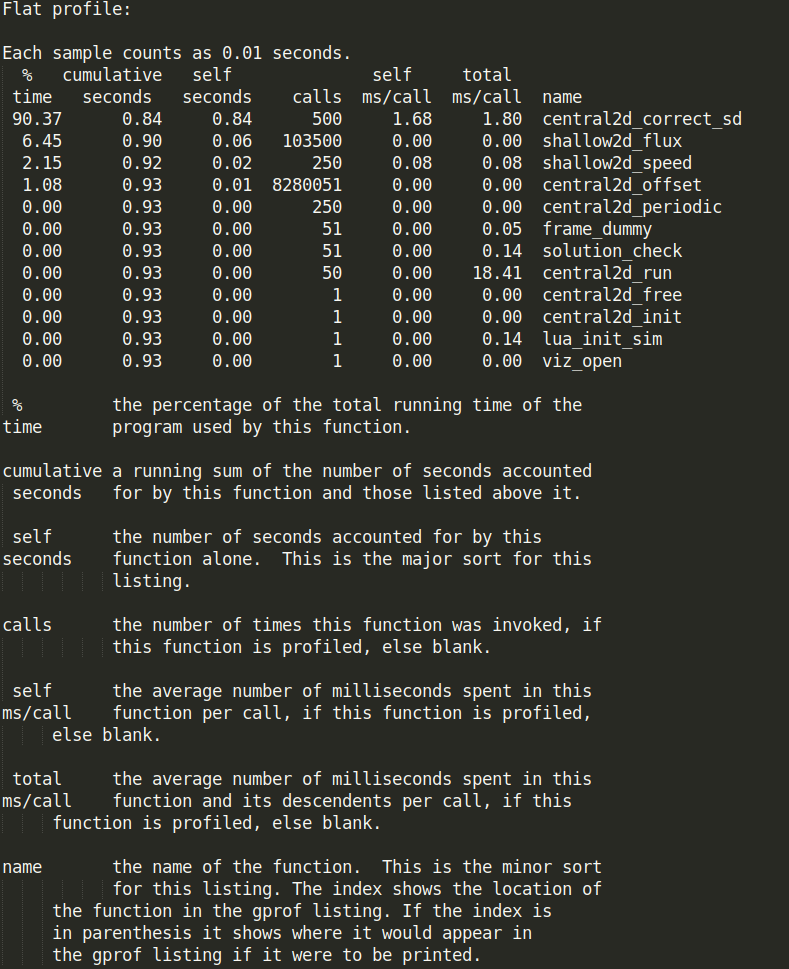
\includegraphics[width=0.8\columnwidth]{../gprof_profile.png}
	\caption{Output from profiling the serial code using gprof.}
	\label{fig:gprof}
\end{figure}

\section{Compilation Details}

Although we used different environments (Mac, Ubuntu, Arch) for local testing, profiling and debugging,
the performance analysis was been done on Graphite. In this section, we discuss the compilation configurations we used.

We used the GCC 5.5.0 compiler provided by Graphite. The four flags that we used for the compilation are the following:
\begin{itemize}
	\item \texttt{-O3} --- Performs more aggressive optimization than \texttt{-O2} used by default.
	\item \texttt{-ffast-math} --- Enables the compiler to reorder operations that may not actually be associative.
	\item \texttt{-fopenmp} --- Enables the OpenMP directive \texttt{\#pragma omp} in our C code for shared memory parallel processing.
	\item \texttt{-march=native} --- Optimizes the code for the specific machine architecture.
\end{itemize}

\section{Conclusion}
To optimize and tune the implementation of the finite volume solver, we have applied two different strategies:
sub-domain partitioning that splits the grid data into sub-grids to ease computation and using OpenMP to parallelize
the computations (each thread handling a sub-grid).
During this process, we overcame two difficulties: maintaining sub-grid consistency and synchronization of $dt$ among the sub-grids.

Our performance analyses suggest that our optimization has doubled the performance with just two processors.
The experiment conducted with strong scaling aligns with Amdahl's Law (that inherently serial part of the code sets the upper bound of the speedup of parallel code),
and the experiments conducted with weak scaling aligns with Gustafson's Law (that the scaled speedup is linear with the number of processors).

Besides the aforementioned approaches, there were two additional attempts that were not as successful.
First, a hybrid OpenMP and MPI strategy would have allowed us to run larger global grids,
yet this approach could not be implemented due to difficulties in rewriting our implementation that does not depend on the global grid and resolving a complicated coordination problem during visualization.
Second, naive insertion of \texttt{\#pragma omp parallel} directive had a significantly worse performance than the serial implementation.

\end{document}
